\documentclass{standalone}
%
\usepackage{tikz}
\usetikzlibrary{backgrounds,shapes.callouts}
\usepackage{tkz-euclide}
\usepackage{xcolor}
\usepackage{ifthen}
%
\definecolor{space}{HTML}{1F2C4E}
\definecolor{earth}{HTML}{0089FA}
\definecolor{dida}{HTML}{FFDE00}
\definecolor{title}{HTML}{FBA706}
\definecolor{moon}{HTML}{AFAFAF}
%
\usepackage{fontspec}
\setmainfont{Open Dyslexic}
%
\title{Il primo cielo non si scorda mai}
\begin{document}
	\tikzset{
		partial ellipse/.style args = {#1:#2:#3}{insert path={+ (#1:#3) arc (#1:#2:#3)}},
		notice/.style  = { draw, ellipse callout, callout relative pointer={#1} },
	}
	\begin{tikzpicture}[background rectangle/.style={fill=white},show background rectangle,>={[inset=0,angle'=27]Stealth}]
		%title
		\draw [black,ultra thick] (1,1) rectangle (29,-1);
		\node at (15,0) {\textcolor{black}{\fontsize{40}{41}\selectfont Il primo cielo non si scorda mai}};
		%\node at (15,11.8) {\textcolor{black}{\fontsize{90}{91}\selectfont del pioniere}};
		%
		\begin{scope}[shift={(0,-5)}]
			\node at (3,0) {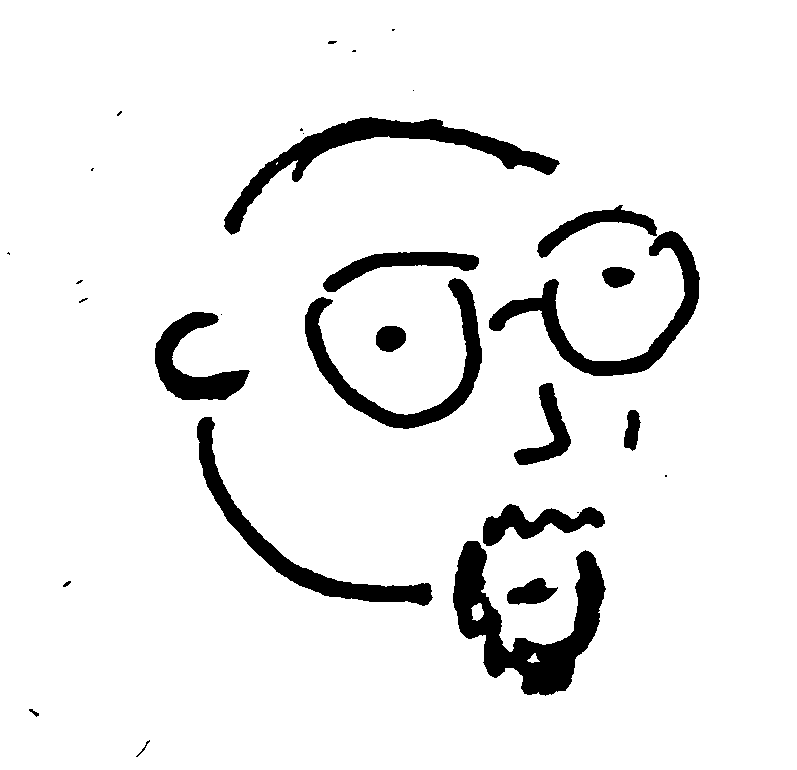
\includegraphics[width=5cm]{img-cielo/io_sx}};
			\node (example-textwidth-2) [right, align=left, text width=22cm, color=black, font=\fontsize{18pt}{19pt}\selectfont] at (6,0) {In una raccolta di storie brevi della \emph{mangaka} \textbf{panpanya}, c'è una paginetta in cui racconta di una sua osservazione notturna del cielo d'inverno!\\Vedeva solo triangoli, come nell'immagine qui sotto!};
		\end{scope}
		% 
		\begin{scope}[shift={(0,-14)}]
			\node at (15,0) {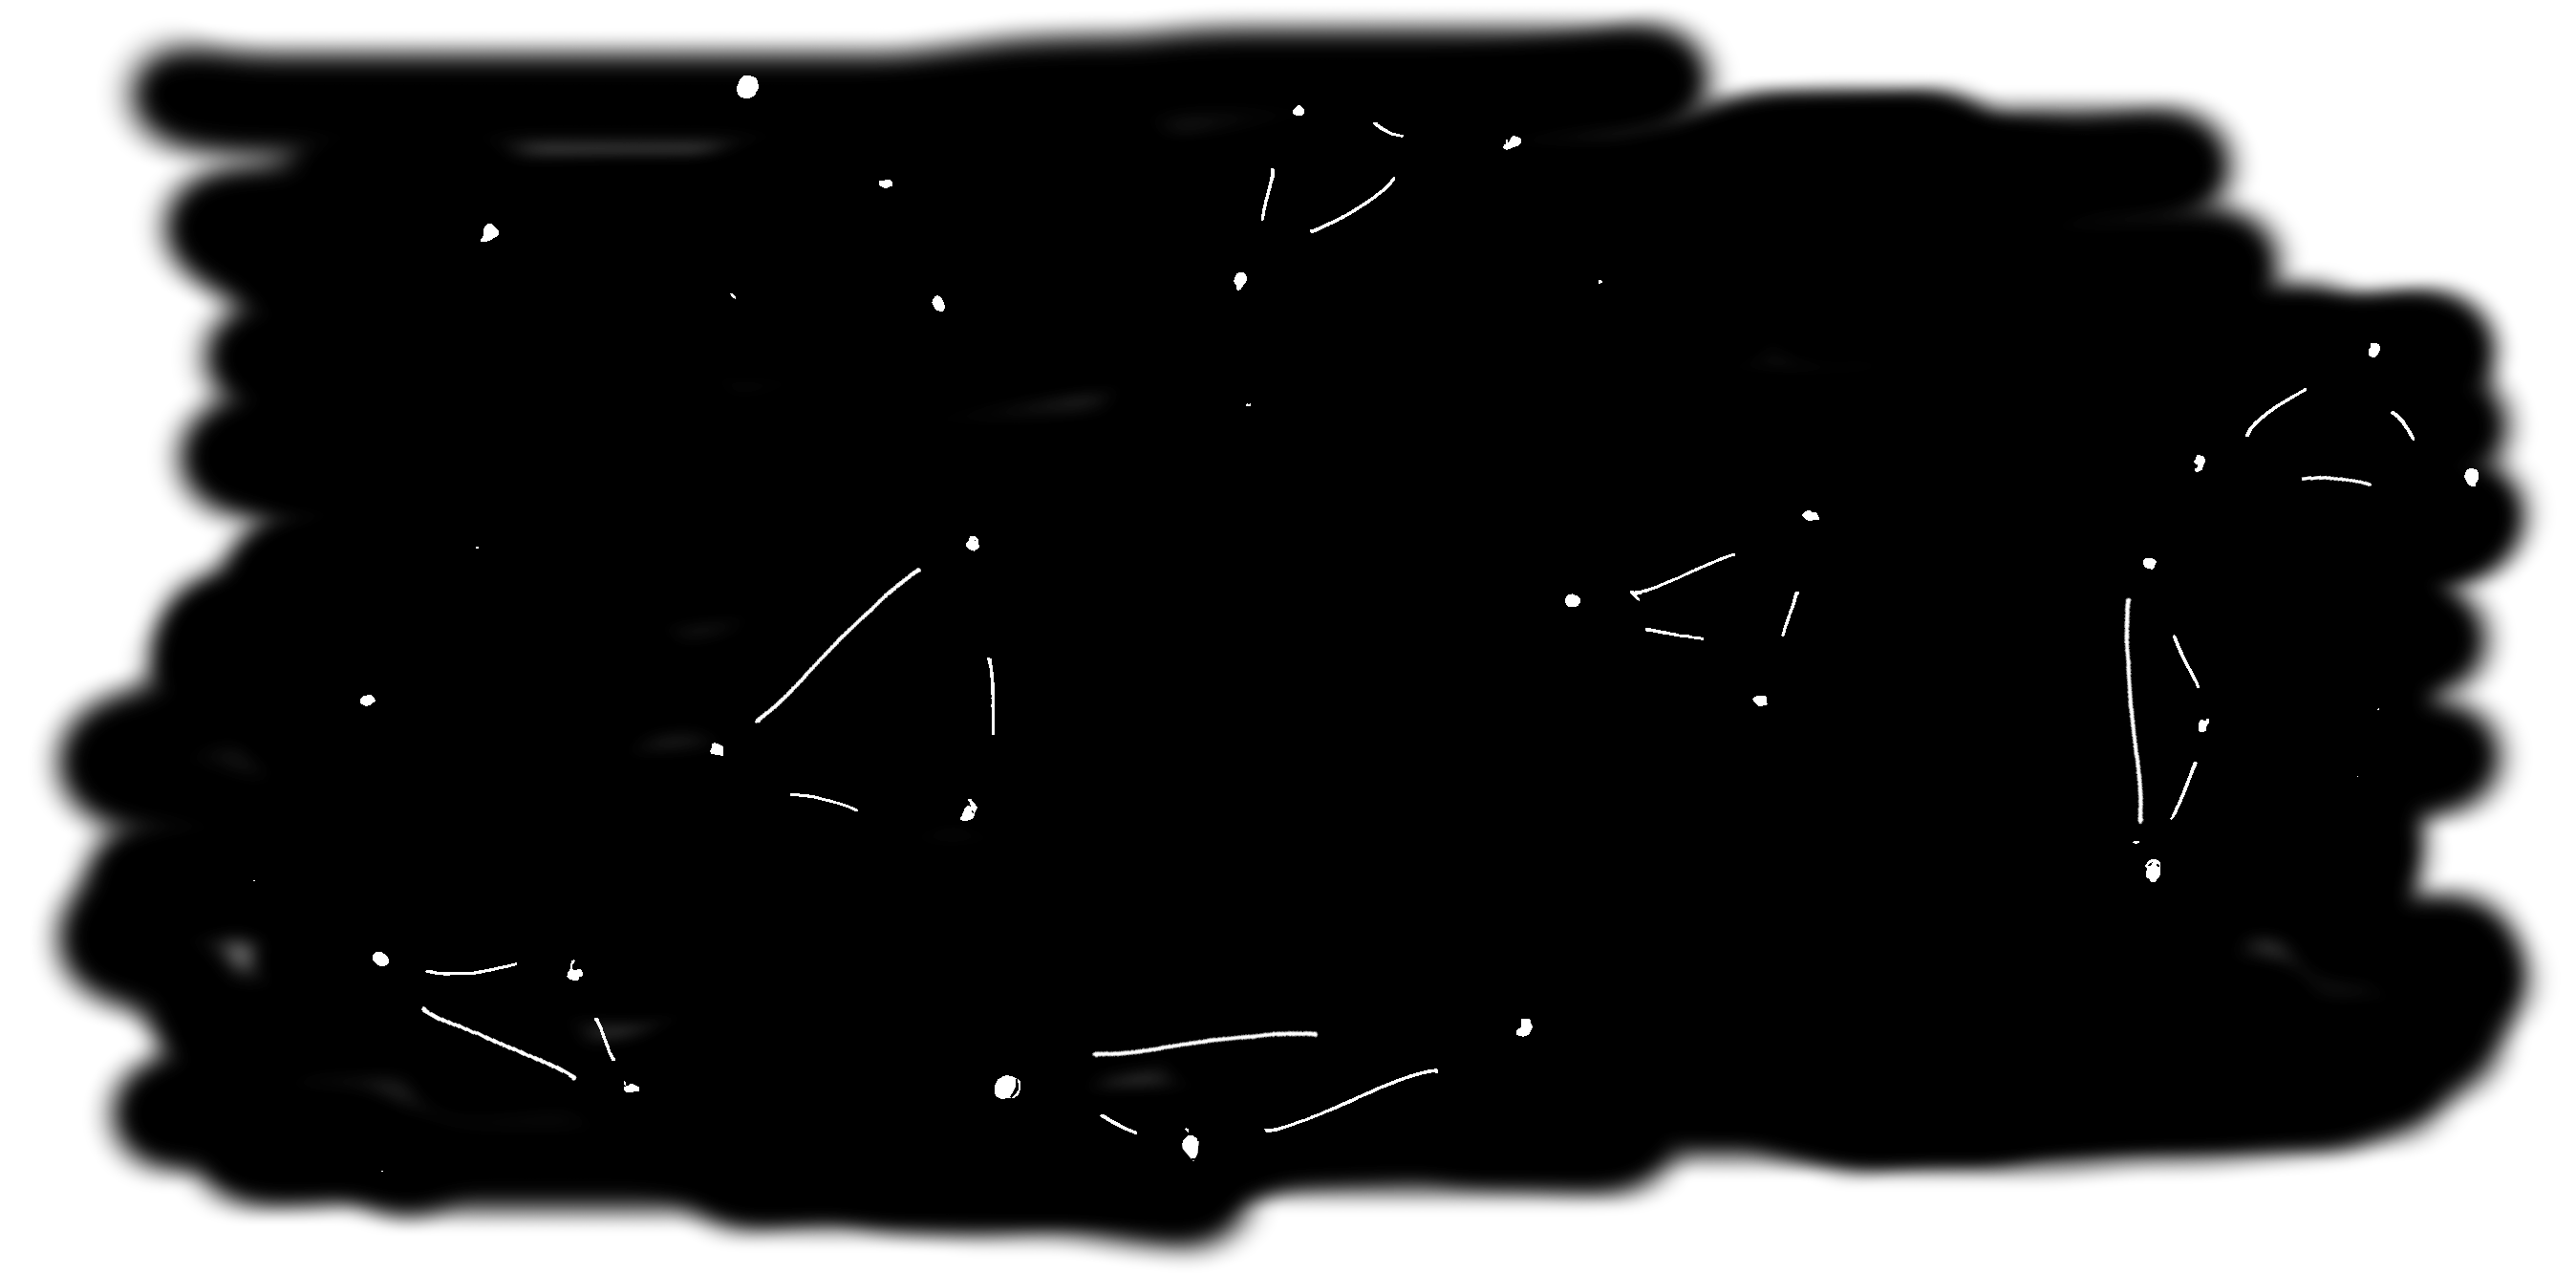
\includegraphics[width=25cm]{img-cielo/stelle-triangoli}};
		\end{scope}
		%
		\begin{scope}[shift={(0,-22)}]
			\node (example-textwidth-2) [right, align=left, text width=28cm, color=black, font=\fontsize{18pt}{19pt}\selectfont] at (2,0) {E mi e' venuta in mente subito la mia prima osservazione di un cielo notturno. In Sila. In Calabria.};
			\node at (15,-6) {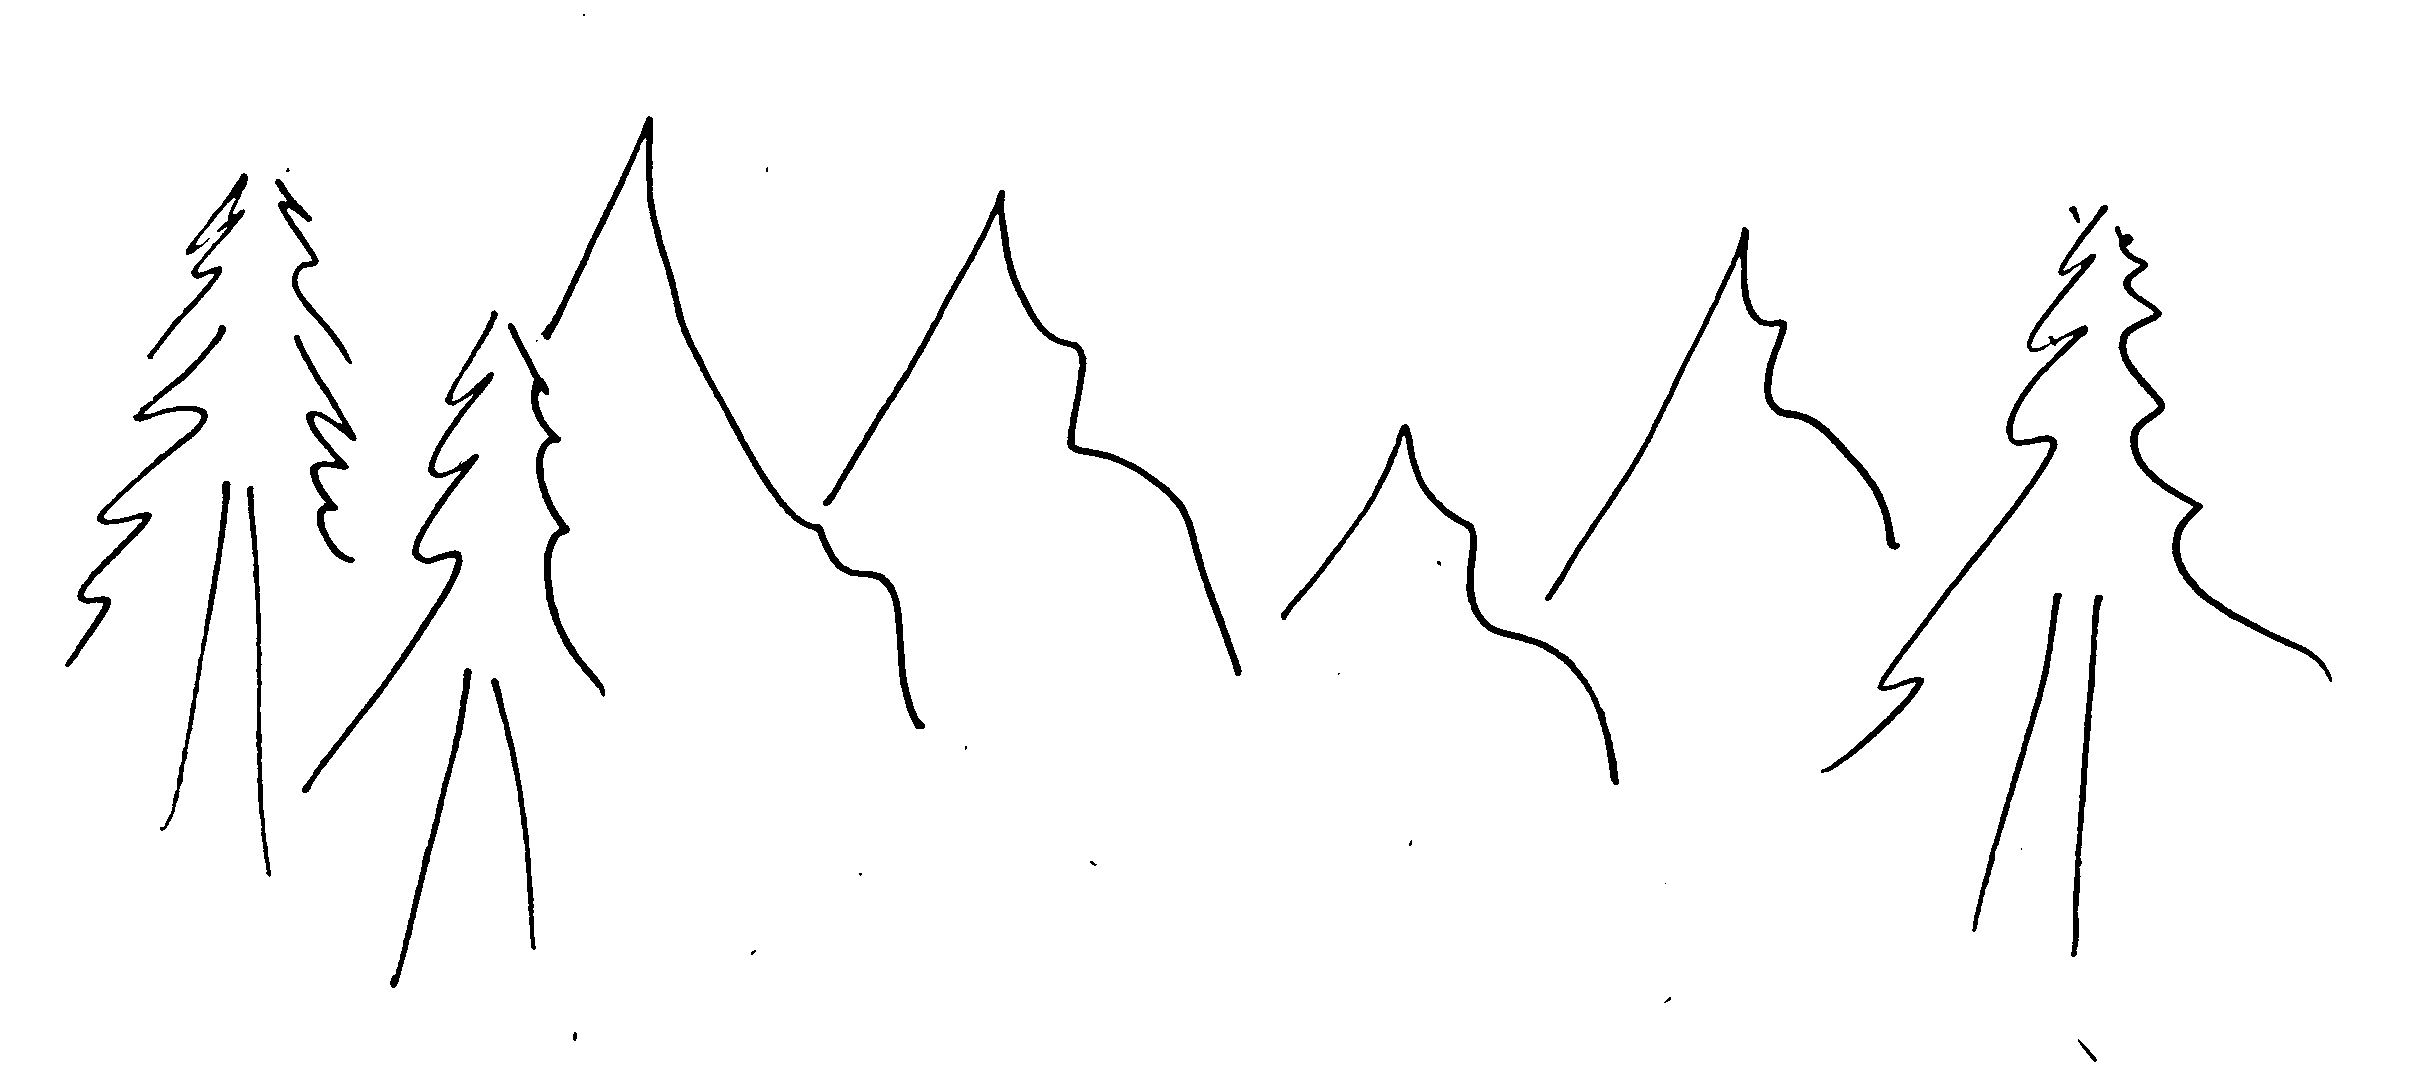
\includegraphics[width=25cm]{img-cielo/paesaggio}};
		\end{scope}
		%
		\begin{scope}[shift={(0,-36)}]
			\node at (23,0) {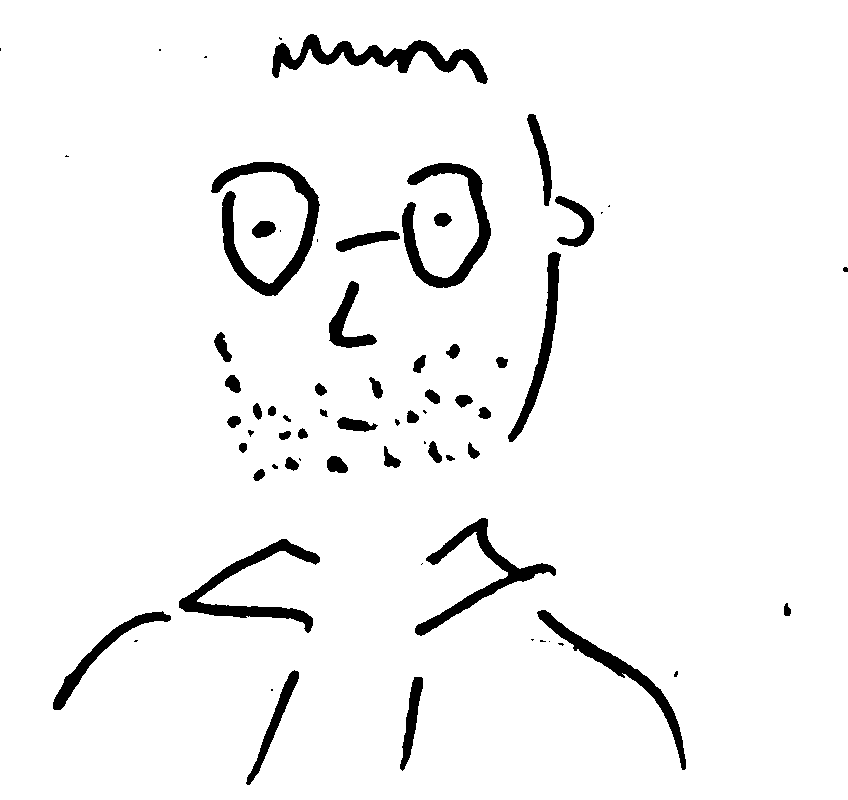
\includegraphics[width=5cm]{img-cielo/io_barba}};
			\node (example-textwidth-2) [right, align=left, text width=18cm, color=black, font=\fontsize{18pt}{19pt}\selectfont] at (2,0) {Ero al liceo, terzo o quarto anno.  Un giovedi' o un venerdi' di primavera (era uno di questi giorni della settimana, visto che gia' all'epoca non mi radevo prima di domenica). A guidarci nell'osservazione c'erano alcuni studenti di fisica dell'Universita' della Calabria, che ci indicavano le stelle e le costellazioni usando delle torce.};
		\end{scope}
		%
		\begin{scope}[shift={(0,-41)}]
			\node at (7,-2) {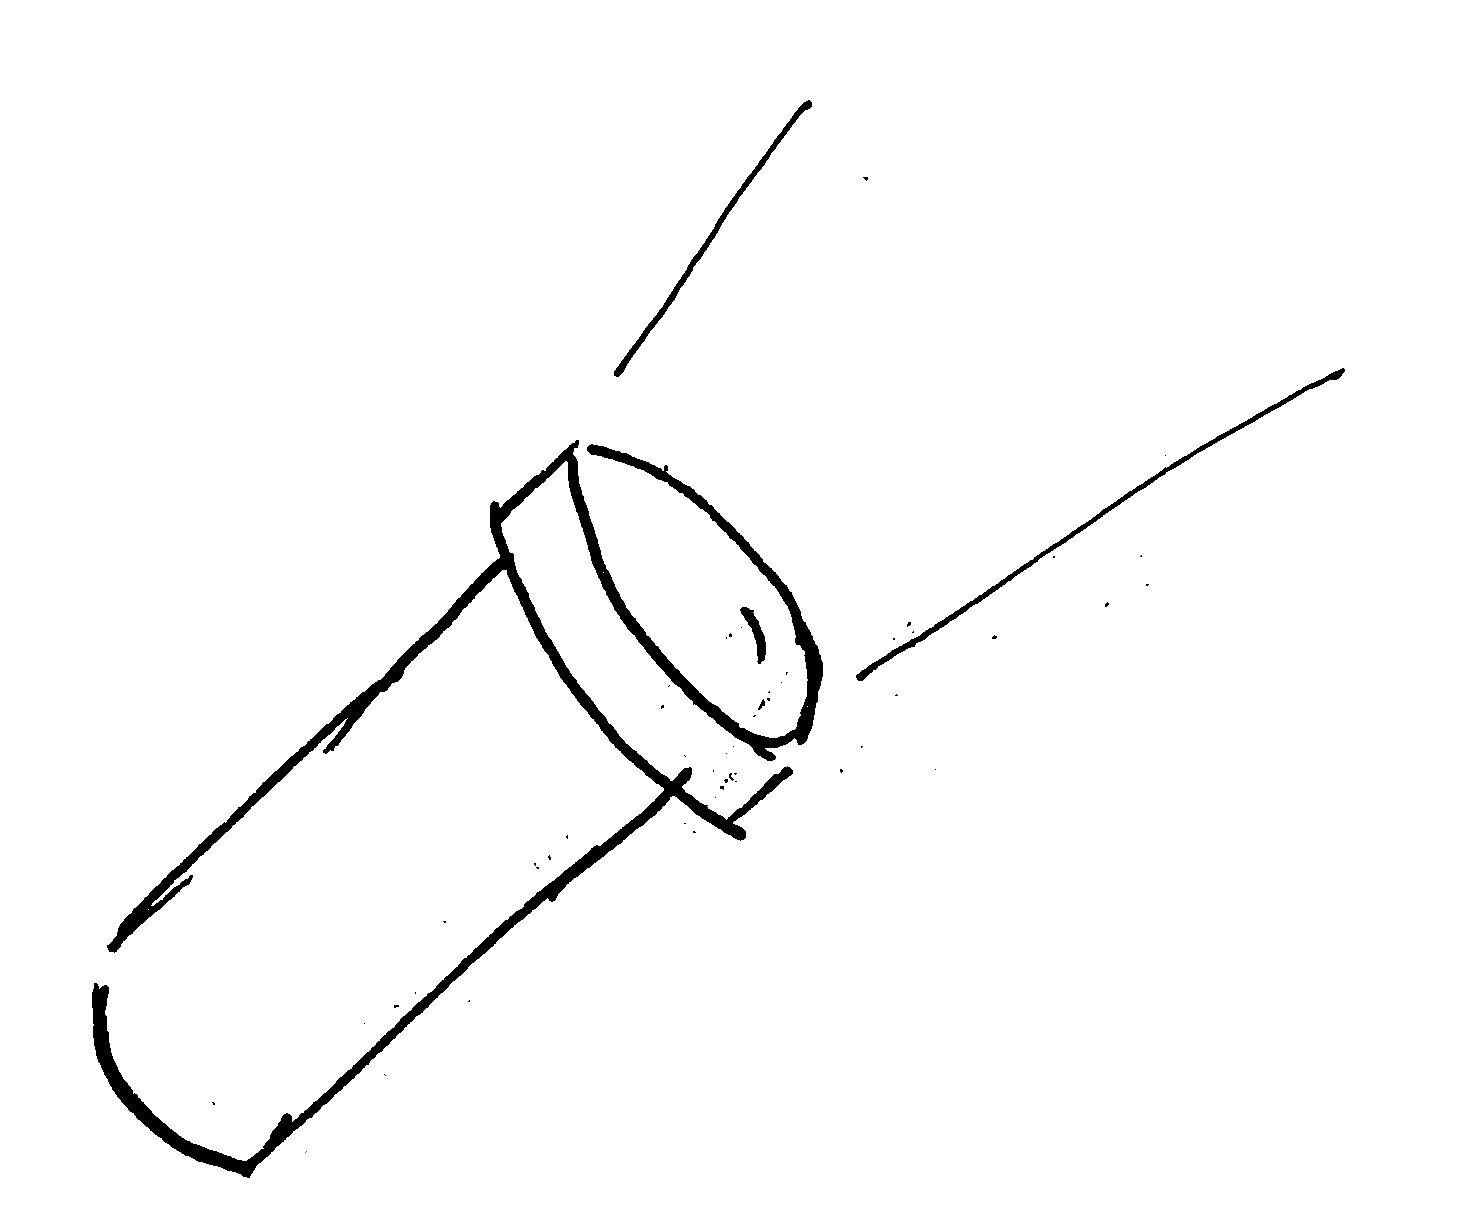
\includegraphics[width=10cm]{img-cielo/torcia}};
			\node (example-textwidth-2) [right, align=left, text width=12cm, color=black, font=\fontsize{18pt}{19pt}\selectfont] at (12,-2) {La luce veniva accesa per pochi secondi, senza rovinare cosi' lo spettacolo delle stelle!};
			\node at (15,-12) {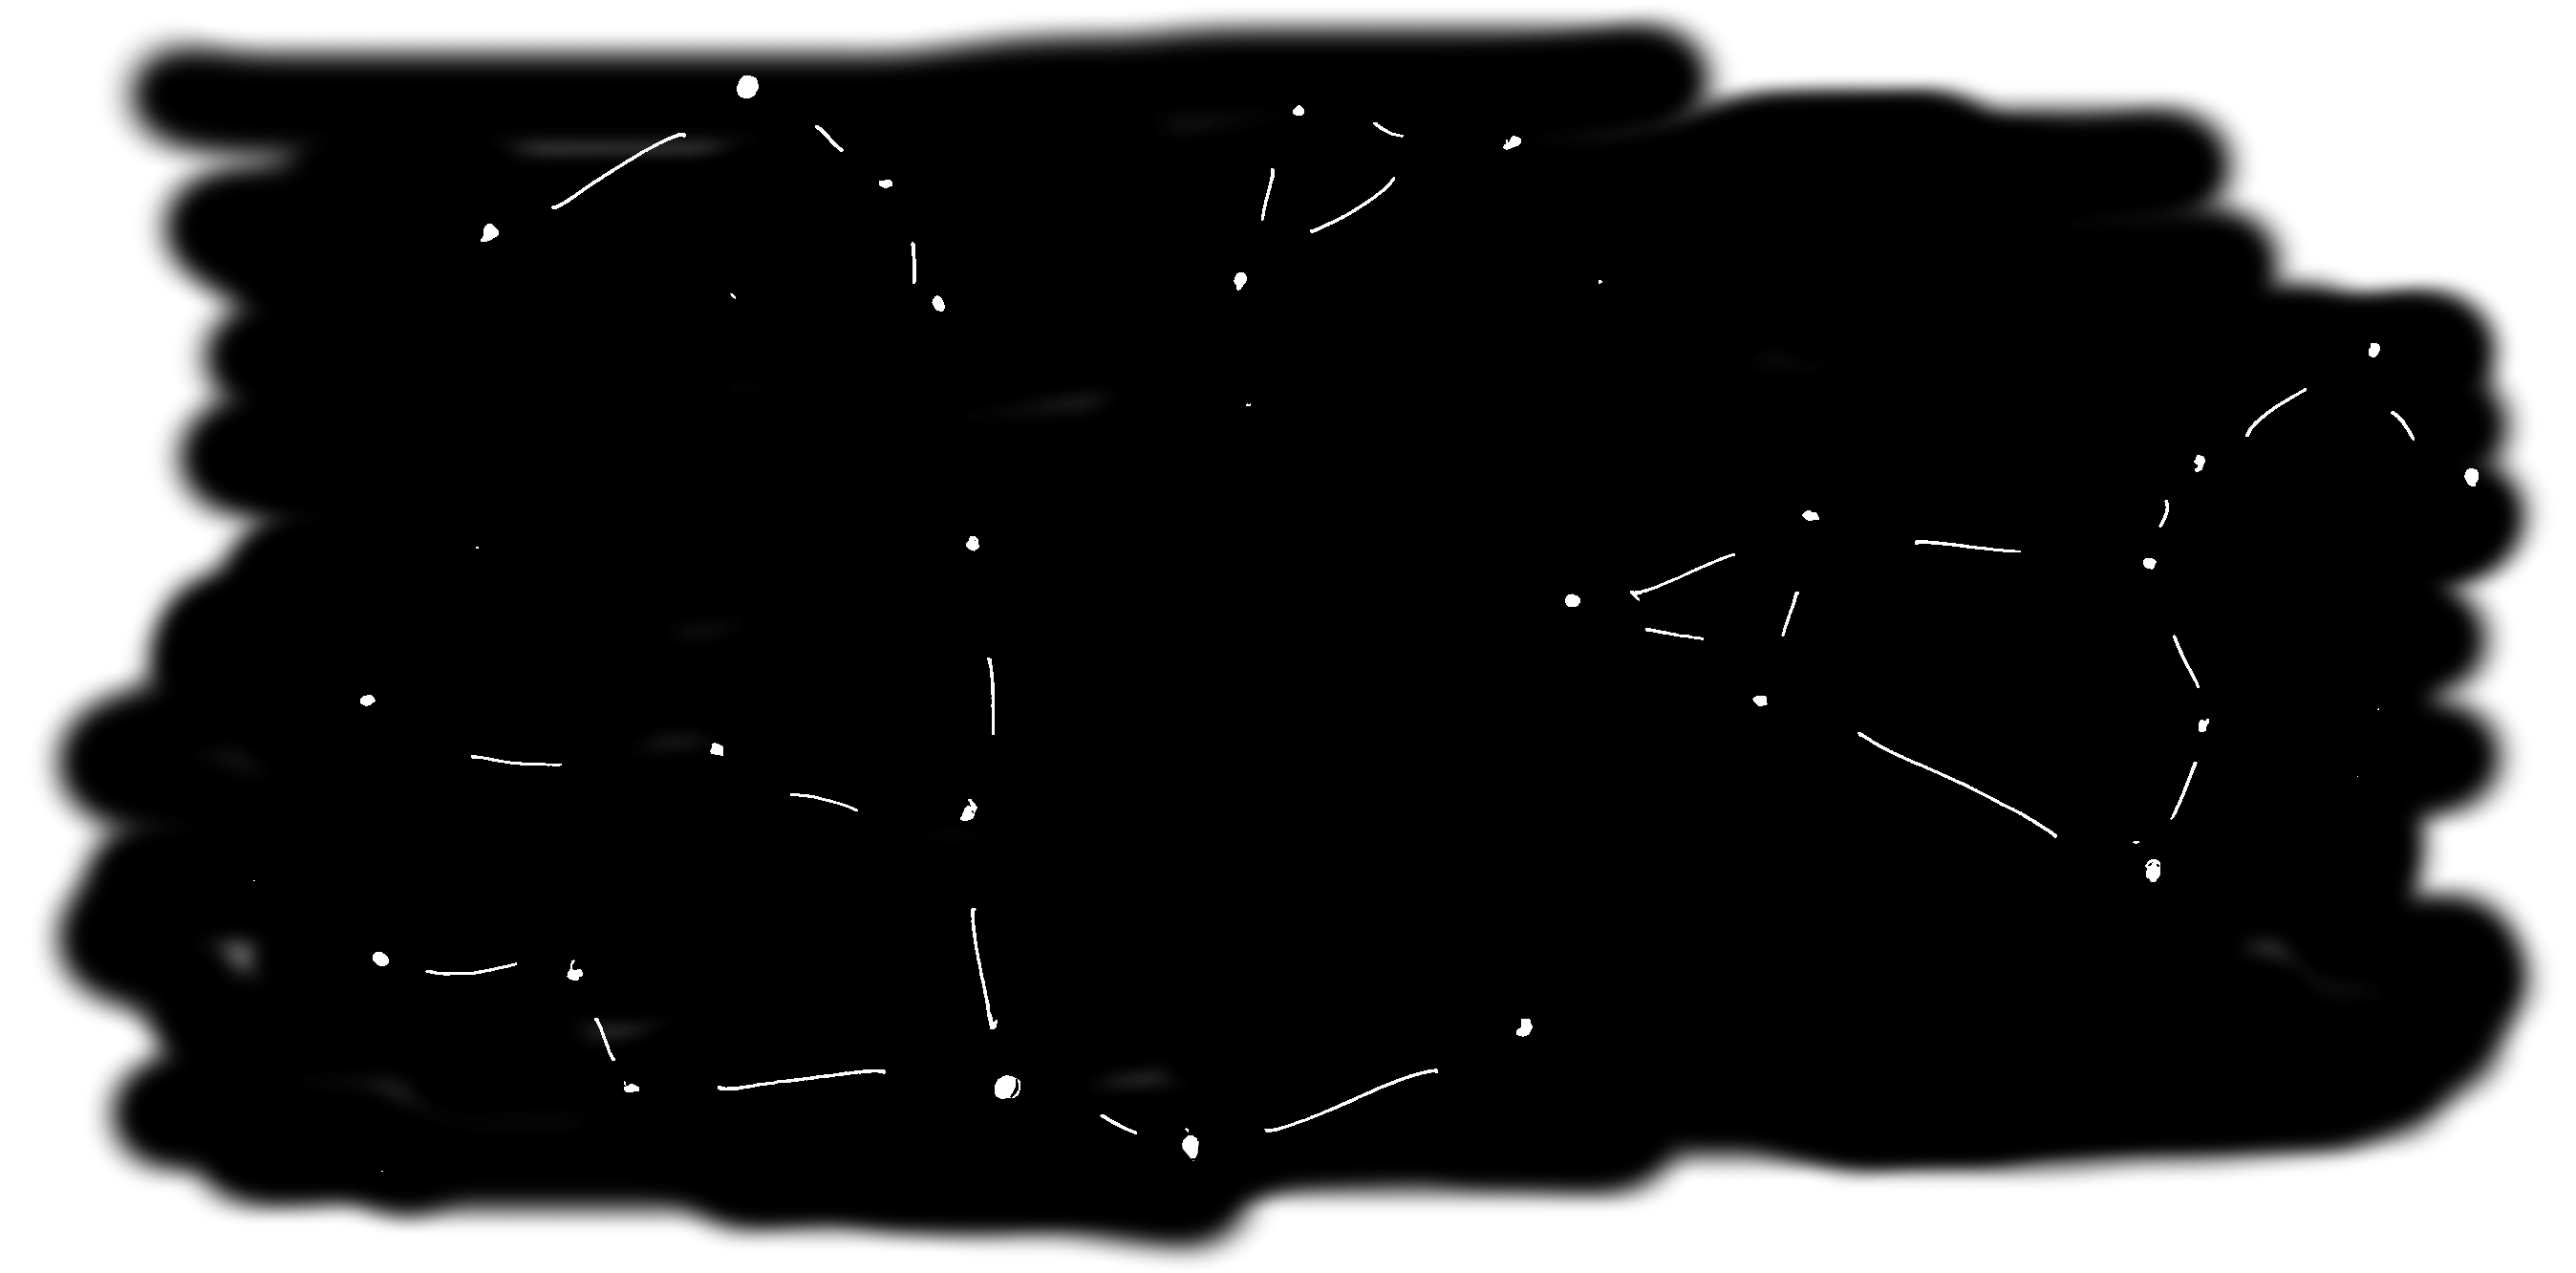
\includegraphics[width=25cm]{img-cielo/stelle-cielo_scuro}};
		\end{scope}
		%
		\begin{scope}[shift={(0,-62)}]
			\node at (23,0) {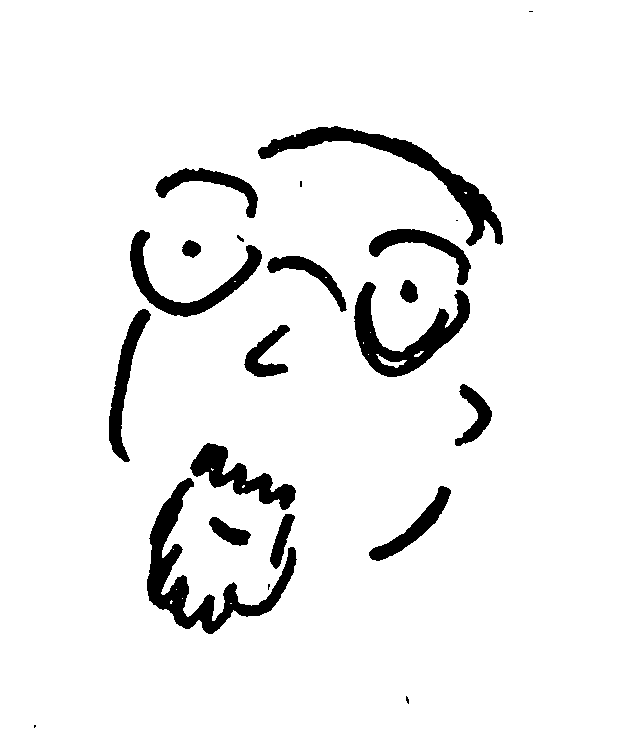
\includegraphics[width=5cm]{img-cielo/io_dx}};
			\node (example-textwidth-2) [right, align=left, text width=18cm, color=black, font=\fontsize{18pt}{19pt}\selectfont] at (2,0) {Fu un'esperienza meravigliosa! E in queste notti d'estate invito tutti i lettori a prendersi il tempo per alzare lo sguardo al cielo notturno. Non solo alla ricerca delle "stelle cadenti"!};
		\end{scope}
		%
		\begin{scope}[shift={(0,-66)}]
			\node at (27,0) () {
\includegraphics[width=3.7cm]{licenza}};
			\node at (15.5,-0.1) {\textcolor{black}{\fontsize{14}{15}\selectfont Testo e illustrazioni, esclusa la placca: @ulaulaman - Gianluigi Filippelli}};
		\end{scope}
	\end{tikzpicture}
%
\end{document}
